\chapter{Introducción}

En la actualidad las redes de datos están creciendo en complejidad. Basta mirar el incremento en la cantidad de aplicaciones web que ofrecen contenido multimedia, para determinar que no sólo crece el volumen de los datos, sino que además se requiere mayor velocidad y confiabilidad en la transmisión. 

También es notoria la consolidación de múltiples servicios sobre redes \mbox{Ethernet,} tales como comunicación de voz, vídeo en estándar y alta definición, videoconferencias, transacciones en tiempo real, etc.

En este contexto es necesario introducir continuas mejoras en el procesamiento de los paquetes de datos. Esto debe darse bajo la premisa de que no alcanza con proveer soluciones rápidas, sino que también se debe dotar a las mismas de un buen grado de flexibilidad y escalabilidad que permitan sostener el ritmo actual de crecimiento en términos de velocidad de procesamiento.



\section{Contexto}


En lo que respecta a las tecnologías de red, las nuevas tendencias se canalizan hacia la agregación de paquetes en flujos. Dos ejemplos los constituyen las redes de conmutación multi-protocolo mediante etiquetas (\textit{Multiprotocol Label Switching}, MPLS) y las redes virtuales  de área local (\textit{Virtual LAN}, VLANs). 

MPLS es un mecanismo en redes de telecomunicaciones de alta performance que transporta datos de nodo a nodo basado en etiquetas en lugar de direcciones de red, con el fin de evitar búsquedas complejas en una tabla de ruteo. Dichas etiquetas se aplican en el inicio de la transmisión e identifican enlaces virtuales entre nodos. También es capaz de encapsular paquetes de varios protocolos de red.

\begin{figure}[h]
  \centering
	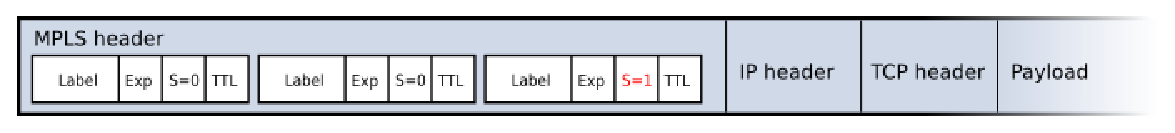
\includegraphics[width=0.99\textwidth]{1-introduccion/graf/MPLS_packet.eps}
  \caption{Encabezado MPLS}
  \label{fig:flow}
\end{figure}
Las VLANs, por otro lado, son redes virtuales, lógicamente independientes, que están conectadas a un mismo conmutador físico. Su funcionamiento se basa en un etiquetado dentro de las tramas de enlace de datos. El estándar IEEE 802.1Q es el que domina el mundo de las VLANs.
\begin{figure}[H]
  \centering
	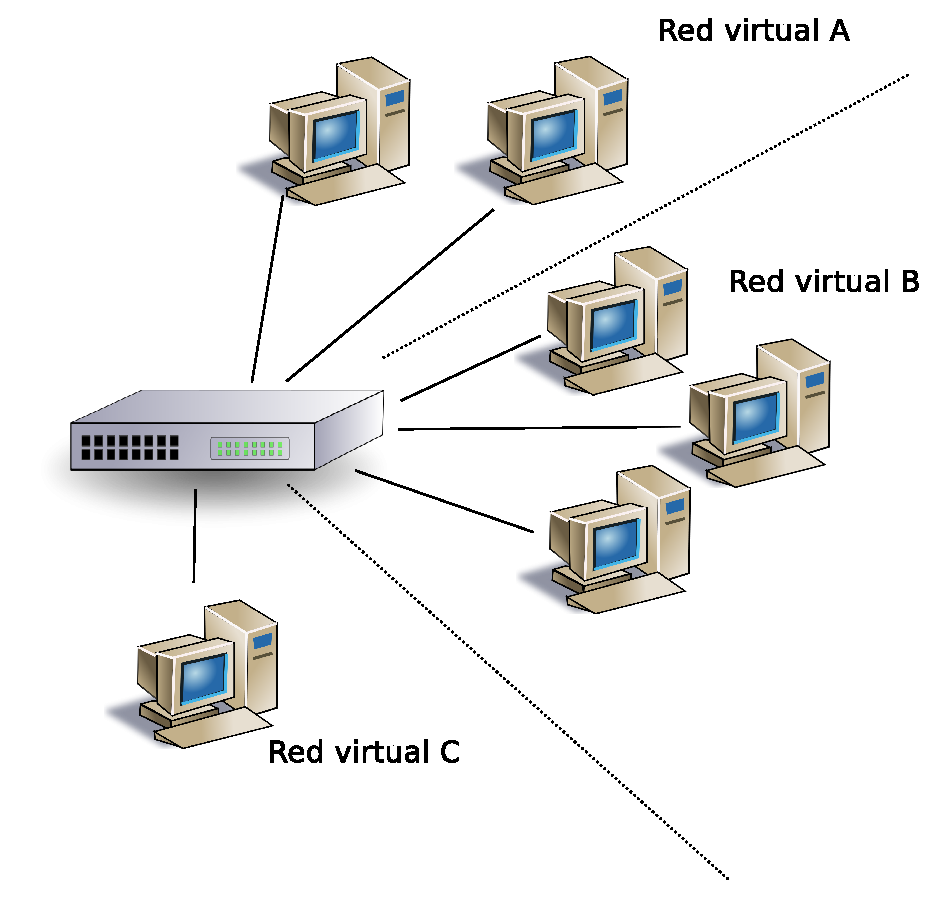
\includegraphics[width=0.90\textwidth]{1-introduccion/graf/vlan.eps}
  \caption{Redes virtuales (VLANs)}
  \label{fig:virt}
\end{figure}

\newpage


En cuanto a las soluciones necesarias para hacer frente a esta brecha entre la necesidad de procesar el flujo creciente y variado de datos de la red y la capacidad de hacerlo, se busca contar con tecnologías que permitan generar respuestas específicas de manera flexible, en el menor tiempo y con el mejor rendimiento posible. Las tecnologías que en la actualidad son usadas para implementar soluciones a estos problemas, son en general tres:

\emph{Los Circuitos Integrados de Propósito Específico (\textit{Application-Specific Integrated Circuit}, ASIC),} están formados por cientos de bloques especializados trabajando en paralelo. Aunque cuentan con un muy buen desempeño, tienen un alto costo inicial y el tiempo para desarrollarlos es grande.

\emph{Los Procesadores de Red (Network Processors, NPs),} específicos para este tipo de problemas, ya que cuentan con múltiples elementos de procesamiento, buena performance para ciertas tareas, aunque tienen dificultades de portabilidad debido a que sus interfaces son propietarias en casi todos los casos.
\begin{figure}[h]
  \centering
      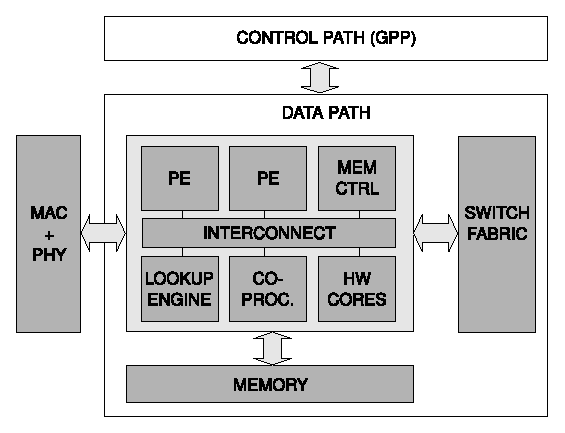
\includegraphics[width=0.8\textwidth]{1-introduccion/graf/NP_based.eps}
  \caption{Solución basada en NP}
  \label{fig:diseno}
\end{figure}
\newpage

\emph{Los Procesadores de Propósito General (General Purpose Processors,GPPs),} utilizan la arquitectura propia de la PC y la adaptan al procesamiento de red mediante un software especializado. Aunque esta solución es muy popular por su flexibilidad y su bajo costo, las transacciones con memoria RAM mediante un bus compartido y la naturaleza secuencial de los GPPs son factores limitantes a tener en cuenta. 
 \begin{figure}[h]
  \centering
      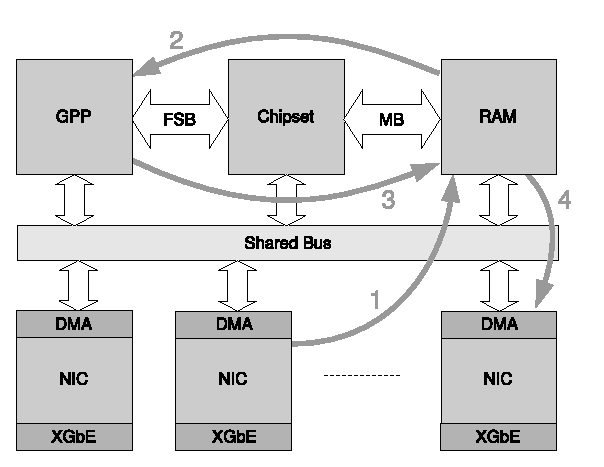
\includegraphics[width=0.8\textwidth]{1-introduccion/graf/GPP_based.eps}
  \caption{Solución basada en GPP}
  \label{fig:diseno}
\end{figure}

Por lo mencionado anteriormente, es notoria la necesidad de encontrar tecnologías que se combinen con las actuales o que cubran sus falencias, para poder satisfacer los requerimientos crecientes de las redes. 

Los FPGAs (Field-Programmable Gate Array) son dispositivos de lógica reconfigurable que es posible programar, una o varias veces, usando un lenguaje de descripción de hardware(\textit{Hardware Description Language}, HDL). Las FPGAs se utilizan en aplicaciones similares a los ASICs; sin embargo son más lentas, tienen un mayor consumo de potencia y no pueden abarcar sistemas tan complejos como los ASICs. A pesar de esto, tienen un flujo de diseño flexible, sus costes de desarrollo y adquisición son mucho menores para pequeñas cantidades de dispositivos y el tiempo de desarrollo es también menor.



Los Sistemas en un Chip (\textit{System on Chip}, SoC) son circuitos integrados que contienen todo, o la mayoría, de los módulos que corresponden a un sistema informático o electrónico en un solo componente. Son usados especialmente en el área de sistemas embebidos. Los microcontroladores son técnicamente SoC, pero se considera que los SoC tienen procesadores más potentes y pueden correr aplicaciones más complejas, para lo cual necesitan mayor cantidad de memoria que suele estar disponible como chips externos. 

Gracias a la disponibilidad en la ultima década de Soft-Core CPUs y otros Soft IP, se ha producido un punto de inflexión en el uso de FPGAs como plataforma para SoC. Como resultado de la combinación de logros técnicos y fuerzas de mercado, varios fabricantes como Altera, Cypress Semiconductor, Intel y Xilinx anunciaron la comercialización de FPGA con facilidades para el desarrollo de SoC.
Estos avances que simplifican el desarrollo de SoC, la flexibilidad en el flujo de diseño y el prototipado rápido son las condiciones que posicionan a las FPGAs como la herramienta indicada para atacar un problema tan complejo como el procesamiento de paquetes en redes de datos.

 \begin{figure}[h]
  \centering
	 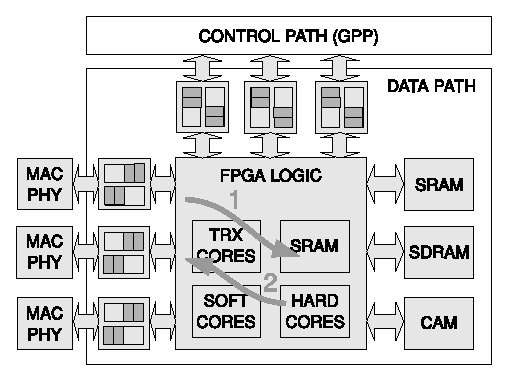
\includegraphics[width=0.8\textwidth]{1-introduccion/graf/FPGA_based.eps}
  \caption{Solución basada en FPGA}
  \label{fig:diseno}
\end{figure}

     




\section{Problema Marco}

Como se mencionó, existe una tendencia a consolidar múltiples servicios sobre un soporte de red como es Ethernet. Asimismo la velocidad de dichas redes está en constante aumento. Esto plantea la necesidad de procesar una mayor cantidad y variedad de paquetes de datos, generando funciones de procesamiento conocidas como \textit{clasificación}. Ésta consiste en la categorización de paquetes en flujos de acuerdo a un conjunto de reglas determinadas. Se efectúa en base a campos en la cabecera del paquete, tales como la dirección IP de origen/destino, puerto de origen/destino, tipo de servicio (TOS), etc. En general, para una clasificación basada en N campos, se dice que ésta es N-dimensional (o multidimensional).

El presente Proyecto Integrador considera en particular el caso de la clasificación unidimensional. Como caso de estudio se toma lo que se conoce como IP lookup, pero la propuesta estudiada en este trabajo puede aplicarse a cualquier caso de dicho tipo de clasificación.

\subsubsection{IP Lookup}

La dirección IP es un número de 32 bits que identifica un dispositivo dentro de una red que utiliza el protocolo IP. Las direcciones IP se suelen representar por cuatro números enteros separados por puntos, que equivalen al valor de cada uno de los cuatro bytes que componen la dirección.
La mayor parte de las redes IP contienen un grupo de direcciones IP jerárquicas. En general se entiende que una parte de la dirección corresponde a la red, y la otra al host dentro de la red. Cuando un dispositivo de enrutamiento recibe un datagrama por una de sus interfaces, compara la parte de red de la dirección con las entradas contenidas en sus tablas y envía el datagrama por la interfaz correspondiente.
Los bits que corresponden a la parte de red conforman lo que se denomina \textit{prefijo de red}.
Existen 3 maneras de representar un prefijo de red:

\begin{itemize}
	\item Binario con asterisco: por ejemplo, el prefijo 132.239 se denotaría 1000010011101111* (dado que 132 es en binario 10000100 y 239 es 11101111). El asterisco al final denota que los bits restantes pueden ser de cualquier valor.
	\item Notación A/L: donde A es una dirección IP y L es la longitud del prefijo. Siguiendo el ejemplo anterior, la notación sería 132.239.0.0/16.
	\item Notación máscara: se utiliza una dirección de red y una máscara en vez de un prefijo explícito. De esta manera, volviendo al ejemplo anteriormente mencionado, este puede expresarse como 132.239.0.0 con máscara 255.255.0.0
\end{itemize}

El procedimiento que se lleva a cabo en un dispositivo de enrutamiento podría describirse de la siguiente manera:

Un paquete llega por una interfaz de entrada. Éste contiene una dirección IP determinada. El dispositivo consulta una tabla para encontrar una interfaz de salida para el paquete en cuestión. Dicha tabla contiene un conjunto de prefijos con sus correspondientes interfaces de salida. El paquete es correspondido con el prefijo más largo que esté contenido en la dirección de destino y luego es redirigido  a la correspondiente interfaz de salida. Esta tarea de determinar el enlace de salida es denominada Búsqueda de dirección (\textit{address lookup).}

En la figura~\ref{fig:prefijos} puede observarse una dirección IP como así también 3 prefijos de diferentes longitudes. Tanto éstos como la dirección están representados por sus bits. En el procedimiento de address lookup la interfaz seleccionada sería aquella asociada al prefijo más largo.

 \begin{figure}[h]
  \centering
	 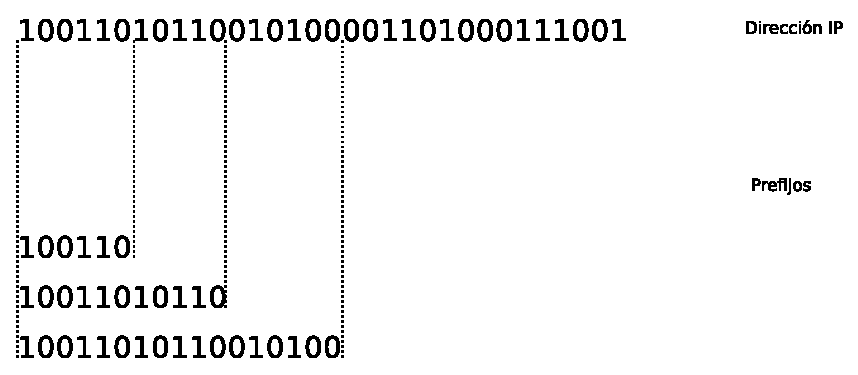
\includegraphics[width=0.7\textwidth]{1-introduccion/graf/prefijos.eps}
  \caption{Dirección IP y prefijos de diferente longitud}
  \label{fig:prefijos}
\end{figure}



\section{Objetivos}
\subsection{Objetivos Generales}
Teniendo en cuenta los problemas planteados, el objetivo general de este proyecto es estudiar los diversos algoritmos de clasificación de paquetes para poder encontrar sus limitaciones en la implementación tanto en software como en hardware. 
En particular, se considera una plataforma de lógica reconfigurable que permite integrar una arquitectura de hardware con software embebido.

\subsection{Objetivos Específicos}
Con el fin de cumplimentar los objetivos generales planteados, son necesarias las siguientes tareas:

    \begin{itemize}     

     	\item Diseñar un sistema embebido que realice la clasificación unidimensional de paquetes mediante una arquitectura mixta hardware-software.
	\item Implementar dicho sistema en hardware reconfigurable.
	\item Implementar al menos 2 algoritmos conocidos y analizar su rendimiento.
	\item Sugerir mejoras en la implementación de los mismos.

\end{itemize}


\section{Organización}

En el capítulo 2 se estudiará, a nivel funcional, una solución propuesta para este tipo de problemas. A continuación, en el capítulo 3, se presentará de manera detallada la arquitectura de los módulos que componen el sistema. En el capítulo 4 se describirá el software. En el capítulo 5 se presentará la integración hardware-software y los recursos utilizados para implementar este proyecto y en el capitulo 6 se presentaran los resultados de esta implementación.






